\documentclass[11pt,a4paper]{article}
\usepackage[margin=18mm]{geometry}
\usepackage{graphicx,booktabs,xcolor,microtype}
\usepackage[T1]{fontenc}
\usepackage{lmodern}
\usepackage{parskip}
\usepackage{enumitem}
\usepackage[hidelinks]{hyperref}
\graphicspath{{report_assets/}}
\definecolor{ink}{HTML}{20313A}
\definecolor{muted}{HTML}{52626A}
\definecolor{accent}{HTML}{2F6B50}
\renewcommand{\familydefault}{\sfdefault}
\setlength{\parskip}{6pt}
\setlist[enumerate]{leftmargin=*,itemsep=3pt,topsep=3pt}
\newcommand{\smallnote}[1]{{\small\color{muted}#1}}
\begin{document}
\color{ink}

{\Large\bfseries Who spoke in the group videos?}\par
\smallnote{Final report on 11 recordings \hfill 29 September 2026}

We wanted a separate voice profile for every numbered person in the videos. We processed all 11 recordings. Eight videos had eight marked faces, and three had seven. That gave us 85 numbered places to fill. The best PSYCON run produced \textbf{57 model-supported profiles}. The other \textbf{28 remain incomplete}.

\begin{center}
\begin{tabular}{l r}
\toprule
Method & Profiles out of 85 \\
\midrule
Original method & 40 \\
NVIDIA method & 13 \\
First PSYCON pass & 45 \\
PSYCON after guarded recovery & \textbf{57} \\
\bottomrule
\end{tabular}
\end{center}

\section*{How we did it}
\begin{enumerate}
\item We took the shared audio from each video and marked the visible faces with numbers.
\item Community-1 found speech turns. Its speaker names were anonymous. It also marked times when people spoke together.
\item TalkNet checked which marked face appeared to speak during each clean turn. SpeechBrain compared the voice across separate turns. We linked a voice to a face only when those checks agreed. A guarded second pass recovered 12 more profiles.
\item We removed overlap and uncertain audio from voice measurements. A profile needed at least three usable seconds and a valid voice embedding. The code built playback clips from the original audio and kept the transcript and other available measurements with each profile.
\end{enumerate}

We tried lower matching thresholds, including 0.42. That shortcut did not safely recover more profiles in the checks we had, so the guarded result is the one we kept. The original and NVIDIA outputs remain available for comparison. Training reads current, ready PSYCON profiles only.

\begin{center}
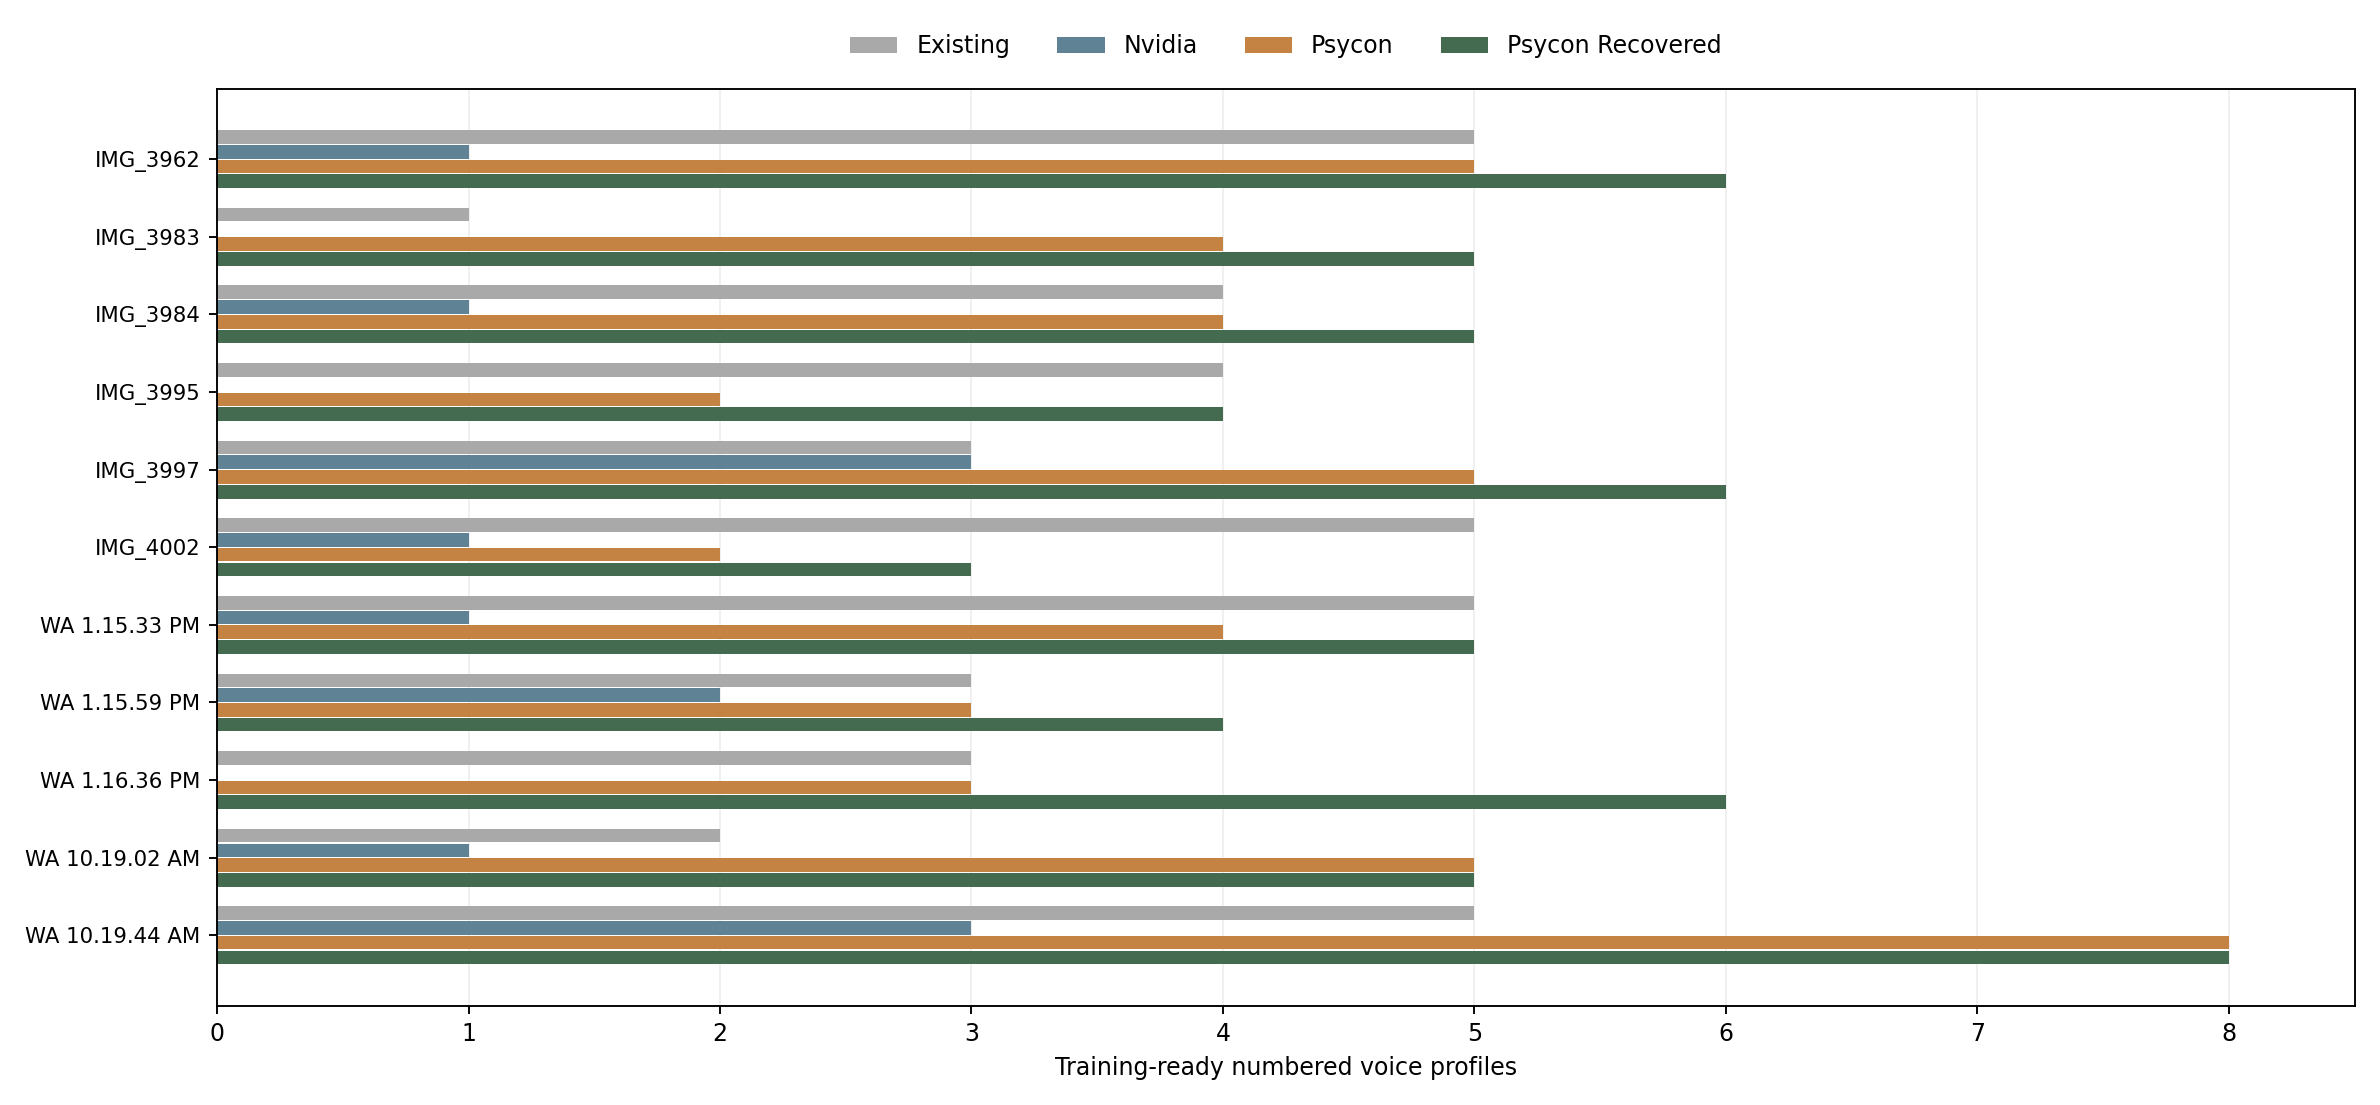
\includegraphics[width=\linewidth,height=70mm,keepaspectratio]{psycon-recovery-comparison.png}\\[-2pt]
\smallnote{Profiles by recording. The green bars show the guarded PSYCON result.}
\end{center}

\clearpage
\section*{What each recording gave us}
\smallnote{WA is short for a WhatsApp video filename. The numbers are profiles that passed each method's own gate, not a measure of identity accuracy.}

\begin{center}
\small
\begin{tabular}{l r r r r r}
\toprule
Recording & Faces & Original & NVIDIA & First PSYCON & Recovered \\
\midrule
IMG\_3962 & 8 & 5 & 1 & 5 & 6 \\
IMG\_3983 & 8 & 1 & 0 & 4 & 5 \\
IMG\_3984 & 7 & 4 & 1 & 4 & 5 \\
IMG\_3995 & 8 & 4 & 0 & 2 & 4 \\
IMG\_3997 & 7 & 3 & 3 & 5 & 6 \\
IMG\_4002 & 8 & 5 & 1 & 2 & 3 \\
WA 1.15.33 PM & 8 & 5 & 1 & 4 & 5 \\
WA 1.15.59 PM & 8 & 3 & 2 & 3 & 4 \\
WA 1.16.36 PM & 7 & 3 & 0 & 3 & 6 \\
WA 10.19.02 AM & 8 & 2 & 1 & 5 & 5 \\
WA 10.19.44 AM & 8 & 5 & 3 & 8 & 8 \\
\midrule
Total & 85 & 40 & 13 & 45 & \textbf{57} \\
\bottomrule
\end{tabular}
\end{center}

\begin{center}
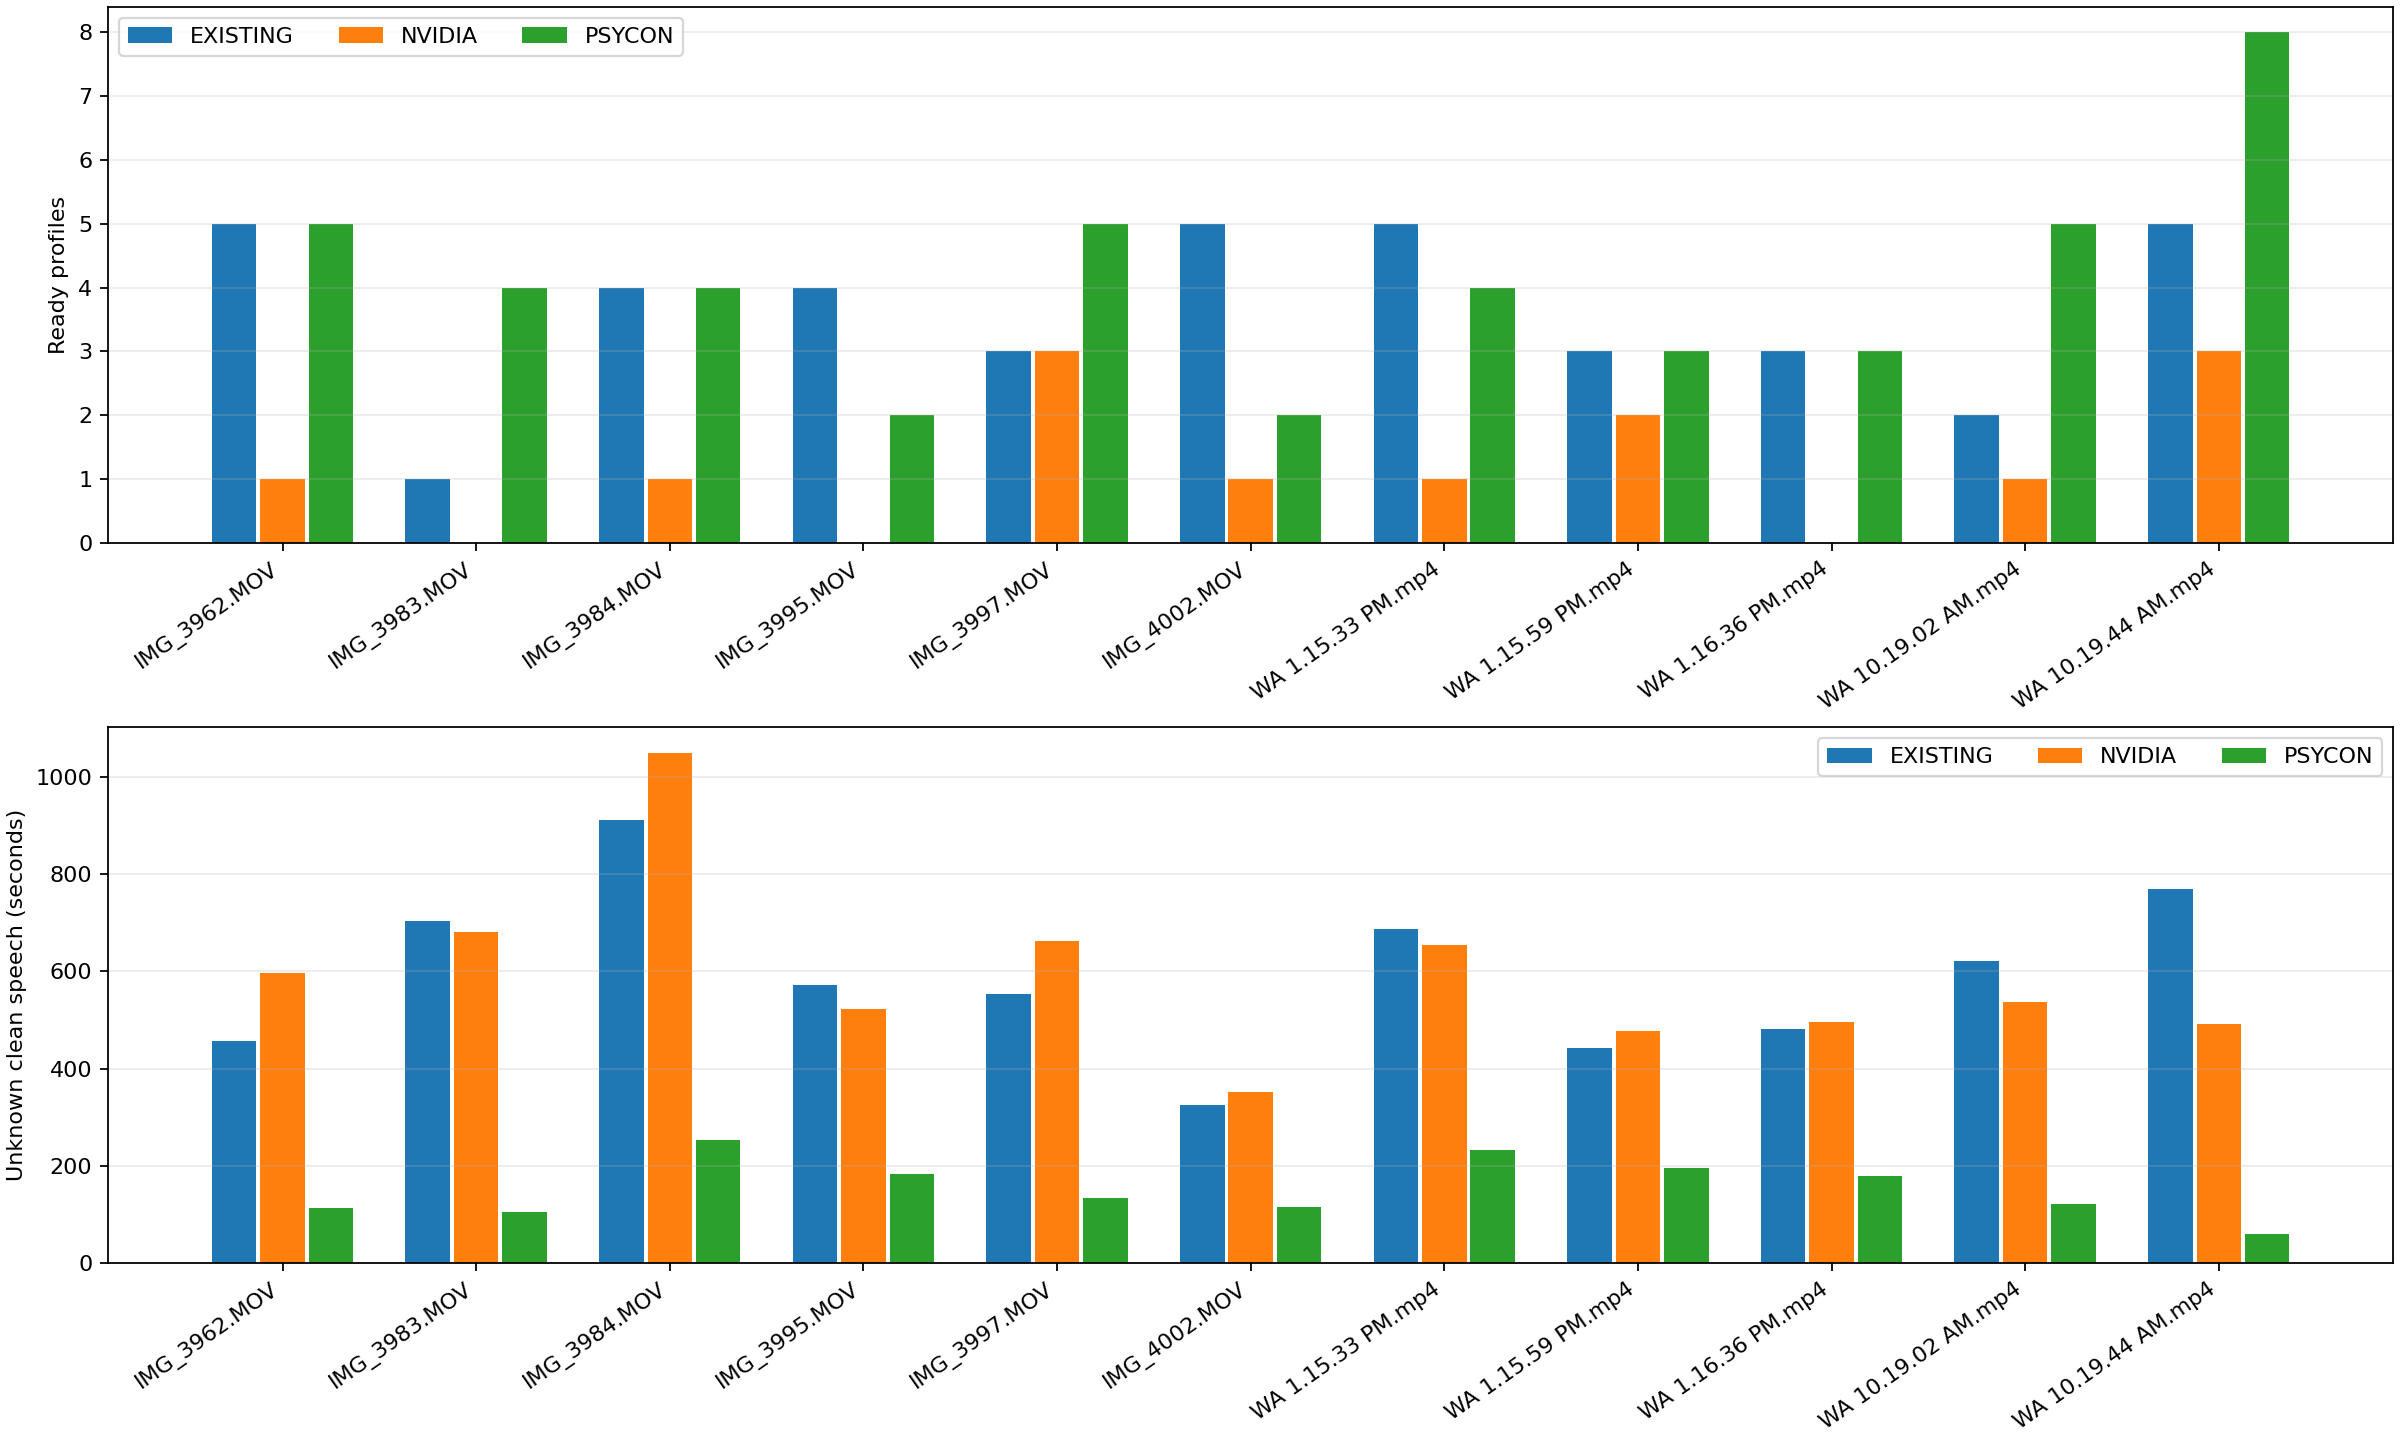
\includegraphics[width=\linewidth,height=112mm,keepaspectratio]{method-comparison.png}\\[-2pt]
\smallnote{The original three-method run. Its PSYCON bars show the first pass, before recovery.}
\end{center}

\clearpage
\section*{What we could not recover}
All 28 incomplete slots have zero \emph{assigned} clean speech. Seventeen have possible TalkNet clips for a person to check. Eleven have no such review candidate. We made 76 PSYCON playback or review clips in total, but nine numbered slots have no person-specific clip that we can defend.

There are 1,420.81 seconds of clean speech that the code could not link to a numbered face. It also found 472.54 seconds of overlapping speech. The original mixed audio can still play back, but it does not go into a single person's voice measurements. The videos also lack a sustained vowel task, so that measurement is unavailable.

We cannot tell whether a particular missing person spoke too little, was hidden from the camera, or was missed by the models. Three recordings have only seven marked faces, so they cannot produce a numbered profile for an unmarked eighth person. The 57 profiles passed model checks, but most were not checked by a person against the full video. Hence we call them \emph{model-supported}, not proven identities.

\begin{center}
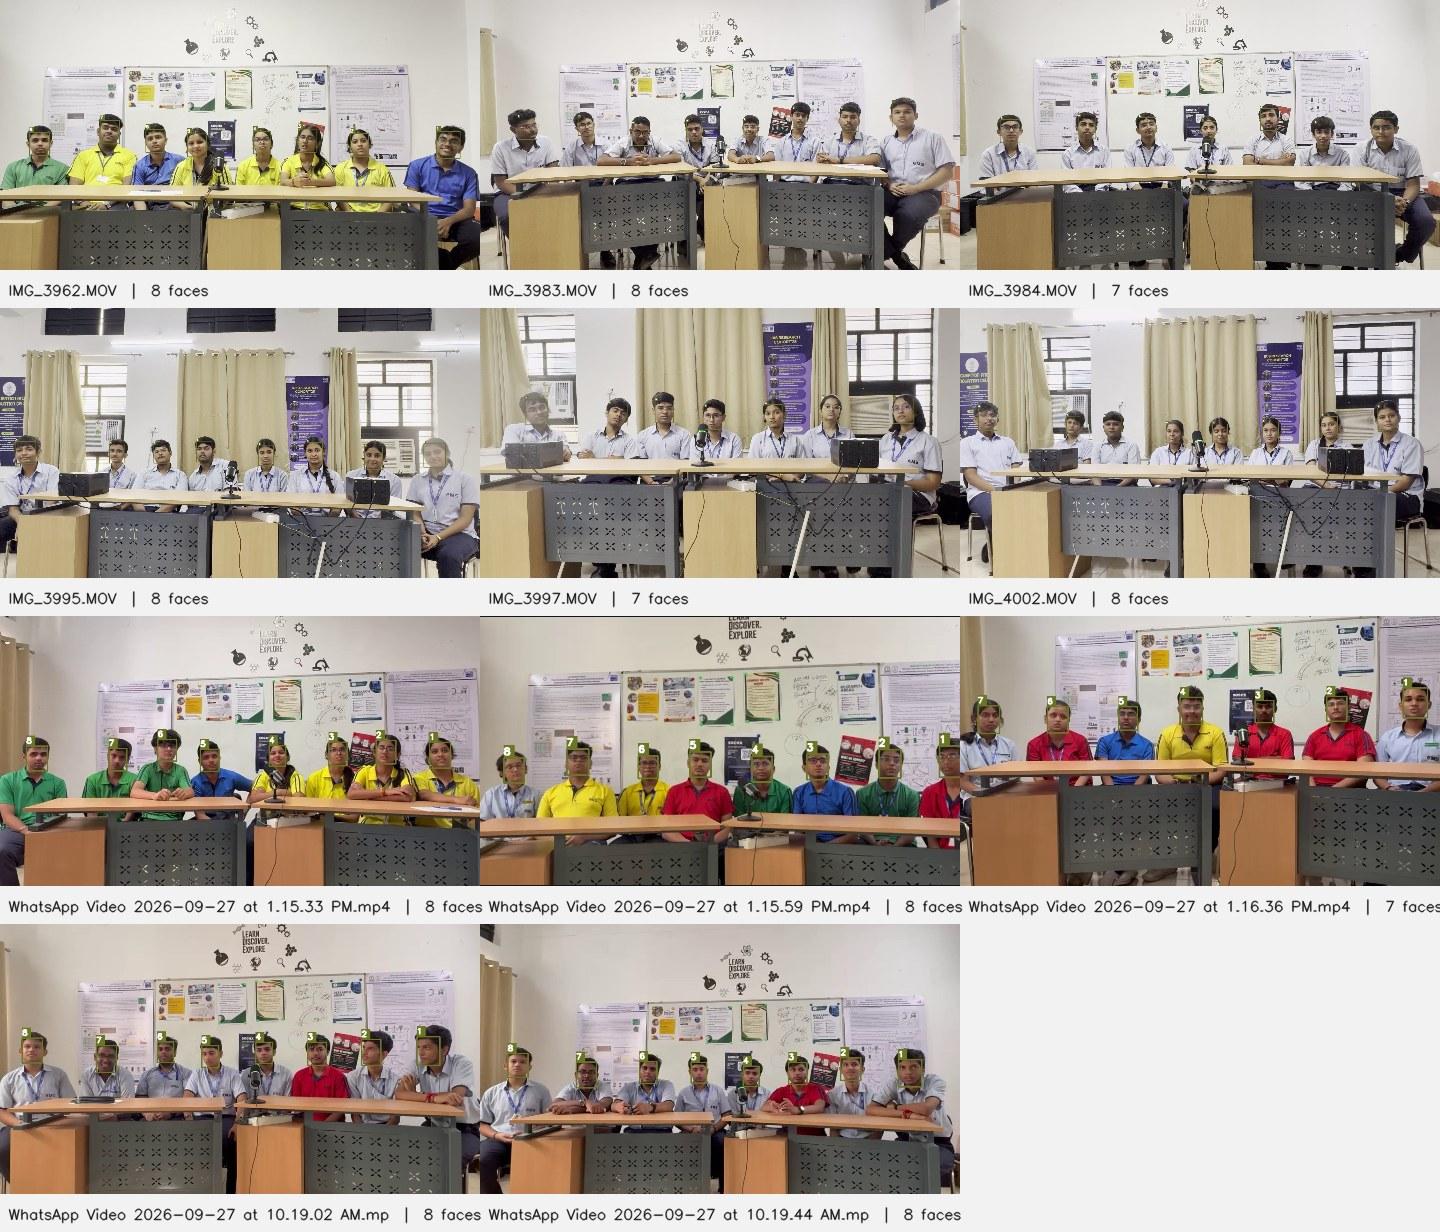
\includegraphics[width=\linewidth,height=139mm,keepaspectratio]{marked-contact-sheet.jpg}\\[-2pt]
\smallnote{The numbered marked frames from all 11 videos. These numbers identify places within each recording.}
\end{center}

\smallnote{Checks: all 44 saved method runs and 223 audio clips passed artifact validation. The full automated test suite passed with six skips. The detailed source intervals and review candidates are in the project audit files.}

\end{document}
